\chapter[Introdução]{Introdução}

Em qualquer sistema de comunicação deve-se garantir uma alta confiabilidade dos dados transmitidos, de forma que no lado do receptor sejam recebidos os mesmos dados enviado pelo transmissor. Esta preocupação ocorre devido aos problemas apresentados nas transmissões como por exemplo: a atenuação do sinal, dessincronização entre o transmissor e o receptor e ruídos apresentados no canal de transmissão \cite{Renato2018}. Para amenizar os efeitos da dessincronização e dos ruídos, desenvolveu-se codificações de linha a fim de aumentar a confiabilidade da transmissão. Dessa forma, torna-se possível a detecção de erros e a implantação de circuitos que sincronizem os dispositivos comunicantes.

Uma codificação inteligente em um canal de transmissão, possibilita transmitir uma maior quantidade de dados por unidade de tempo \cite{Comer2016}. Estas codificações são extremamente úteis em sistemas para física de altas energias. Nestes sistemas, há a presença de um clock elevado e um interesse de uma alta confiabilidade no canal, implicando na necessidade de implementação de uma codificação no canal de transmissão. Esta codificação possibilita a introdução de mecanismos para identificar possíveis erros, com a inserção de circuitos corretores de erros, além de possibilitar que circuitos externos sincronizem os dispositivos comunicantes.

\section{Motivação}

Este trabalho é parte de uma colaboração com o laboratório “São Paulo Research and Analysis Center” (SPRACE) \cite{Sprace2018}. O laboratório SPRACE possui vários ramos de pesquisa, sendo uma delas a instrumentação eletrônica para os sistemas do LHC. O LHC tem uma extensão de 27 km de circunferência, localizado na fronteira Franco-Suiça, tendo por objetivo descobrir a origem da massa das partículas elementares e outras dimensões do espaço \cite{Wikipedia2018}. O colisor é o maior equipamento já construído para pesquisa em física de altas energias do mundo, obtendo resultados expressivos como a descoberta do Bóson de Higgs. Este Bóson é uma partícula elementar prevista pelo modelo padrão de partículas, que ajuda a explicar a massa de outras partículas elementares \cite{Randal2013}.

No percurso do colisor há 4 detectores : ATLAS, CMS, Alice, e LHCb. O acelerador de partículas fornece velocidade e os detectores captam os produtos do impacto das partículas. Dessa forma, pode-se observar a existência de traços de partículas elementares que explicam teorias importantes sobre a física de altas energias \cite{Ferreira2009}. Na \autoref{lhc} é ilustrado um esquema do grande colisor de Hádrons que está localizado a 175 metros abaixo do solo.

\begin{figure}[H]
	\caption{\label{lhc} Esquema do grande colisor de Hádrons (LHC).}
	\centering
	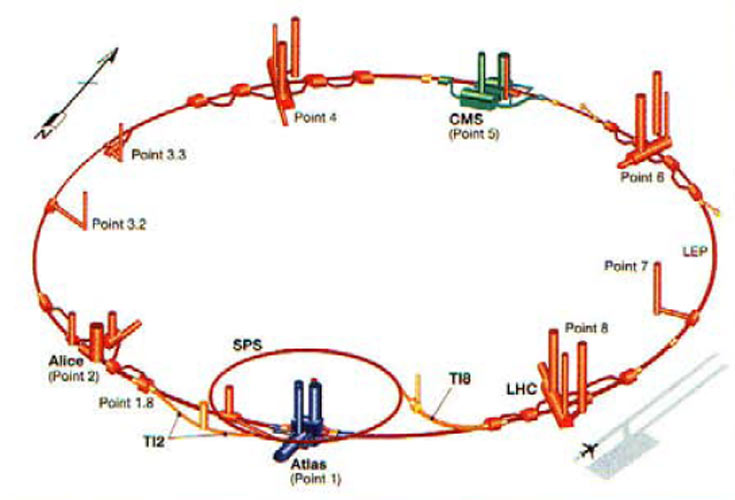
\includegraphics[scale=0.5]{lhc.jpg}
	\begin{center}
		Fonte: Elaborado pelo Autor
	\end{center}	
\end{figure}

O grande colisor está em um processo de pesquisa para realizar uma grande atualização, a chamada "Grande Luminosidade". Desta forma, a instrumentação existente no colisor deve ser atualizada para suportar o novo volume de dados gerados. Os sistemas desenvolvidos devem serem capazes de transmitir e processar um grande volume de dados em uma faixa muito curta de tempo \cite{Lucio2018}. 

O trabalho desenvolvido pelo laboratório SPRACE está diretamente ligado ao detector “Solenóide de Muon Compacto” (CMS) do LHC. Os detectores do LHC tem estruturas diferentes e cada um obtém dados de partículas específicas. A junção de todos os dados de todos os detectores forma uma imagem completa do experimento, ajudando a realizar novas descobertas. 

O detector CMS tem 6 metros de diâmetro e 13 metros de comprimento captando ao longo do diâmetro as posições das partículas. Dessa forma, é possível traçar o caminho das partículas por produzirem dados de posições ao longo do diâmetro do detector. As partículas carregadas seguirão caminho em espiral no campo magnético de 4 Tesla (T) do detector possibilitando calcular os seus momentos, uma vez que momentos diferentes indicam partículas diferentes. Portanto, por meio desses dados é possível coletar evidências para comprovar teorias de novas partículas \cite{Emanuel2018}.

A colaboração entre o laboratório SPRACE com o CMS objetiva-se colaborar no desenvolvimento de sistemas na área da instrumentação eletrônica, o qual serão implementados dentro de um sistema completo de detecção. O novo sistema que está em desenvolvimento, principalmente objetiva-se eliminar as restrições de latência que o atual possui \cite{Cms2018}.

\section{TRABALHO DESENVOLVIDO}

No ambiente do detector há uma alta taxa de radiação eletromagnética, por conta da alta velocidade dos átomos presentes no tubo. Dessa forma, em transmissões de alta velocidade de uma placa para outra podem acarretar a presença de ruídos no canal de transmissão. Os ruídos presentes no canal de transmissão danificam os dados originais, acarretando no armazenamento de dados incoerentes para um posterior estudo. Portanto, uma codificação presente no canal de transmissão possibilita a detecção de erros e a solução de problemas envolvidos na transmissão em altas velocidades, como por exemplo a dessincronização entre o transmissor e o receptor.

Este trabalho desenvolve o estudo da codificação 64b66b e suas características por meio do Simulink($MATLAB^{TM}$). Dessa forma, o sistema desenvolvido pode ser usado como codificação do canal de transmissão entre duas placas FPGA garantindo uma maior confiabilidade dos dados transmitidos.

O trabalho confeccionado foi dividido em 7 partes. No \autoref{teo:filds} é apresentado uma noção geral sobre campos finitos, teoria essencial para o entendimento dos sistemas presentes na codificação. No \autoref{teo:lfsr} é apresentado a teoria dos \textit{Linear FeedBack Shift Registes (LFSR)}, componente essencial para os \textit{Cyclic Redundancy Check (CRC)} e os \textit{scramblers}. No \autoref{teo:scrambler} é apresentado a teoria dos \textit{scramblers}, sistemas essenciais para garantir o balanço entre os bits 1's e 0's na transmissão. No \autoref{crc:teoria} é apresentado a teoria dos CRC's, sendo os responsáveis pela detecção de erro no dado transmitido. A codificação 64b66b é descrita no \autoref{codificacao64b66b}, bem como todos os componentes para realizar a transmissão do dado. No \autoref{sys:teo} é apresentado a descrição do sistema desenvolvido com a codificação 64b66b. No \autoref{concu:teo} é apresentado algumas simulações e conclusões sobre o funcionamento do sistema desenvolvido.
